\documentclass[10pt, a4paper]{article}

\usepackage[margin=1.5cm, top=1.8cm, bottom=1.8cm]{geometry}
\usepackage{xcolor}
\usepackage{tikz}
\usepackage{enumitem}
\usepackage{multicol}
\usepackage{parskip}
\usepackage{titlesec}
\usepackage{fancyhdr}
\usepackage{microtype}
\usepackage{mdframed}
\usetikzlibrary{shapes.geometric, arrows.meta, positioning, fit, backgrounds, calc}

% Colors
\definecolor{cblue}{RGB}{25, 70, 150}
\definecolor{cgreen}{RGB}{20, 110, 60}
\definecolor{cgray}{RGB}{90, 90, 90}
\definecolor{clightblue}{RGB}{220, 232, 255}
\definecolor{clightgreen}{RGB}{220, 245, 225}
\definecolor{clightyellow}{RGB}{255, 250, 220}
\definecolor{clightorange}{RGB}{255, 235, 210}
\definecolor{clightred}{RGB}{255, 225, 220}
\definecolor{clightgray}{RGB}{245, 245, 245}
\definecolor{cgrayline}{RGB}{190, 190, 190}

% Section style
\titleformat{\section}{\small\bfseries\color{cblue}}{}{0em}{}[\vspace{-4pt}\color{cgrayline}\hrule\normalcolor\vspace{2pt}]
\setlength{\columnsep}{0.8cm}

% Header
\pagestyle{fancy}
\fancyhf{}
\lhead{\textcolor{cgray}{\tiny Travel AI Governance --- PoC One-Pager}}
\rhead{\textcolor{cgray}{\tiny Connector $\times$ VeUP \ | \ April 2026 \ | \ Confidential}}
\renewcommand{\headrulewidth}{0.3pt}
\setlength{\headheight}{14pt}

% =============================================
\begin{document}
\setlength{\parskip}{3pt}

% ---- TITLE -------------------------------------------
{\centering
  {\large\bfseries\color{cblue} Travel AI Governance --- PoC Brief}\par
  \vspace{2pt}
  {\small\color{cgray} What the client needs. What Connector delivers. What I will build.}\par
}
\vspace{6pt}

% ---- TWO COLUMNS: Problem + Deliver ------------------
\begin{multicols}{2}

\section{What I Understood}

\begin{itemize}[leftmargin=*, itemsep=1pt, topsep=2pt, label=\textcolor{cblue}{\small$\bullet$}]
  \item Travel platform uses AI for search, booking recommendations, and CRM --- all live and customer-facing
  \item Every AI interaction today is a disposable log --- no governance, no enforcement, no chain of custody
  \item If a regulator asks ``why did your AI suggest this?'' --- they cannot answer that today
  \item User consent exists but is \textbf{not enforced} at AI execution time --- it is a database field, not a gate
  \item High-value bookings have no human review step --- AI acts unilaterally regardless of amount
  \item They want a \textbf{sidecar} --- nothing ripped, nothing replaced, governance runs alongside
  \item Must be AWS-native --- everything in their own account, no SaaS data exposure
  \item The PoC deliverable is two files: \texttt{traveler\_profile.md} and \texttt{trip\_details.md} --- compiled from governed event history
  \item The real long-term value is warm-start personalisation --- AI remembers context across sessions
  \item GDPR, CCPA, and EU AI Act (Aug 2025) make this a legal requirement, not just a nice-to-have
\end{itemize}

\vspace{4pt}
\section{What I Can Deliver}

\begin{itemize}[leftmargin=*, itemsep=1pt, topsep=2pt, label=\textcolor{cgreen}{\small$\checkmark$}]
  \item \textbf{Capture API} --- REST endpoint that ingests search and booking events from their Python/Node app
  \item \textbf{3 Live Policies} --- consent check, \$5K booking threshold $\to$ HITL, PII field redaction
  \item \textbf{Tamper-evident audit chain} --- every decision CID-addressed, Ed25519 signed, append-only
  \item \textbf{Memory compilation} --- governed events compiled into structured \texttt{.md} profile files
  \item \textbf{Replay demo} --- given user ID + date, produce signed proof of what AI saw and decided
  \item \textbf{Grafana dashboard} --- live policy decisions and audit events via webhook
  \item \textbf{Terraform deploy} --- one-command setup in their AWS account (ECS Fargate)
\end{itemize}

\end{multicols}

% ---- ARCHITECTURE DIAGRAM ----------------------------
\vspace{4pt}
\section{PoC Architecture --- Connector as Governance Sidecar}
\vspace{6pt}

\begin{center}
\begin{tikzpicture}[
  font=\footnotesize,
  box/.style={rectangle, rounded corners=3pt, minimum width=2.4cm, minimum height=0.7cm, text centered, draw, thick},
  arrow/.style={-{Stealth[length=5pt]}, thick, color=cgray},
  dasharrow/.style={-{Stealth[length=5pt]}, thick, dashed, color=cgrayline},
  label/.style={font=\tiny, color=cgray},
]

% ---- Travel App (left side) ----
\node[box, fill=clightyellow, draw=orange!60, text width=2.2cm] (app) at (0, 0)
  {\textbf{Travel App}\\\tiny Python / Node.js};

\node[box, fill=clightyellow, draw=orange!60, text width=2.2cm, below=0.5cm of app] (ai)
  {\textbf{AI Model}\\\tiny GPT-4 / Bedrock};

\node[box, fill=clightyellow, draw=orange!60, text width=2.2cm, below=0.5cm of ai] (crm)
  {\textbf{CRM / Booking}\\\tiny Existing systems};

% Brace label for travel app
\node[font=\tiny\bfseries, color=orange!80!black, left=0.1cm of app, rotate=90, anchor=south] {\small Client Stack};

% ---- Connector Sidecar (center) ----
\begin{scope}[on background layer]
  \node[rectangle, rounded corners=5pt, fill=clightblue, draw=cblue, thick,
    minimum width=7.4cm, minimum height=5.6cm]
    (sidecar) at (5.5, -1.2) {};
\end{scope}

\node[font=\tiny\bfseries\color{cblue}] at (5.5, 1.55)
  {CONNECTOR SIDECAR \ (ECS Fargate --- Client AWS Account)};

% Capture
\node[box, fill=white, draw=cblue, text width=2.0cm] (capture) at (4.0, 0.8)
  {\textbf{Capture API}\\\tiny /v1/capture/search\\/v1/capture/booking};

% Admission Gate
\node[box, fill=clightred, draw=red!50, text width=2.2cm] (gate) at (7.0, 0.8)
  {\textbf{Admission Gate}\\\tiny 5-layer guard pipeline\\deny-by-default};

% Policy Engine
\node[box, fill=clightyellow, draw=orange!50, text width=2.0cm] (policy) at (4.0, -0.4)
  {\textbf{Policy Engine}\\\tiny consent check\\booking threshold\\PII redaction};

% Memory Kernel
\node[box, fill=clightgreen, draw=green!50!black, text width=2.0cm] (kernel) at (7.0, -0.4)
  {\textbf{Memory Kernel}\\\tiny redb storage\\CID-addressed\\Ed25519 signed};

% Surface Engine
\node[box, fill=clightblue, draw=cblue!60, text width=2.0cm] (surface) at (4.0, -1.6)
  {\textbf{Surface Engine}\\\tiny memory compilation\\time-travel query\\proof packages};

% HITL
\node[box, fill=clightorange, draw=orange!70, text width=2.0cm] (hitl) at (7.0, -1.6)
  {\textbf{HITL Queue}\\\tiny high-value review\\\$5K+ bookings};

% Audit Storage
\node[box, fill=clightgray, draw=cgray, text width=4.6cm, minimum height=0.6cm] (audit) at (5.5, -2.7)
  {\textbf{Audit Chain} \ \ (append-only, CID-addressed, signed receipts)};

% ---- Output (right side) ----
\node[box, fill=clightgreen, draw=cgreen, text width=2.4cm] (profile) at (10.8, 0.3)
  {\textbf{traveler\_profile.md}\\\tiny preferences, consent\\interaction history};

\node[box, fill=clightgreen, draw=cgreen, text width=2.4cm] (trip) at (10.8, -0.8)
  {\textbf{trip\_details.md}\\\tiny trip context, decisions\\audit reference};

\node[box, fill=clightblue, draw=cblue, text width=2.4cm] (grafana) at (10.8, -1.9)
  {\textbf{Grafana Dashboard}\\\tiny live policy events\\consent states};

\node[box, fill=clightyellow, draw=orange!60, text width=2.4cm] (replay) at (10.8, -3.0)
  {\textbf{Replay Proof}\\\tiny regulator query\\signed package};

% ---- Arrows: Travel App → Sidecar ----
\draw[arrow] (app.east) -- node[above, label]{SDK capture} (capture.west);
\draw[dasharrow] (ai.east) -- ++(0.8,0) -- ++(0,0.95) -- (capture.west);
\draw[dasharrow] (crm.east) -- ++(0.8,0) -- ++(0,1.95) -- (capture.west);

% ---- Arrows: Within Sidecar ----
\draw[arrow] (capture.east) -- (gate.west);
\draw[arrow] (gate.south) -- (kernel.north);
\draw[arrow] (capture.south) -- (policy.north);
\draw[arrow] (policy.east) -- (kernel.west);
\draw[arrow] (policy.south) -- (surface.north);
\draw[arrow] (kernel.south) -- (hitl.north);
\draw[arrow] (surface.east) -- (hitl.west);
\draw[arrow] (surface.south) -- ++(0,-0.3) -- (audit.west);
\draw[arrow] (hitl.south) -- ++(0,-0.3) -- (audit.east);

% ---- Arrows: Sidecar → Outputs ----
\draw[arrow, color=cgreen] (surface.east) -- ++(1.2, 0) -- (profile.west);
\draw[arrow, color=cgreen] (surface.east) -- ++(0.9, 0) -- ++(0,-0.8) -- (trip.west);
\draw[arrow] (audit.east) -- ++(0.6, 0) -- ++(0, 0.8) -- (grafana.west);
\draw[arrow] (audit.east) -- ++(0.6, 0) -- ++(0, -0.3) -- (replay.west);

% ---- Labels ----
\node[font=\tiny\bfseries, color=cgreen, right=0.1cm of profile, rotate=270, anchor=north] {\small Outputs};
\node[font=\tiny, color=cgray, below=0.1cm of audit] {S3 export for long-term retention};

\end{tikzpicture}
\end{center}

\vspace{4pt}
% ---- FOOTER ROW ----
\noindent
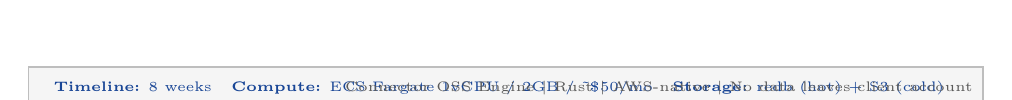
\begin{tikzpicture}[font=\tiny]
  \fill[clightgray] (0,0) rectangle (\linewidth, 0.55cm);
  \draw[cgrayline] (0,0) rectangle (\linewidth, 0.55cm);
  \node[anchor=west, color=cblue] at (0.2, 0.28)
    {\textbf{Timeline:} 8 weeks \ \ \textbf{Compute:} ECS Fargate 1vCPU / 2GB / \textasciitilde\$50/mo \ \ \textbf{Storage:} redb (hot) + S3 (cold)};
  \node[anchor=east, color=cgray] at (\linewidth - 0.2, 0.28)
    {Connector OSS Engine $|$ Rust $|$ AWS-native $|$ No data leaves client account};
\end{tikzpicture}

\end{document}
